\documentclass{softwaremanual}

\usepackage{titling}

% Figures and controlling packages
\usepackage{float}
\usepackage{wrapfig}

% logo for the title page
\newcommand{\swlogo}{{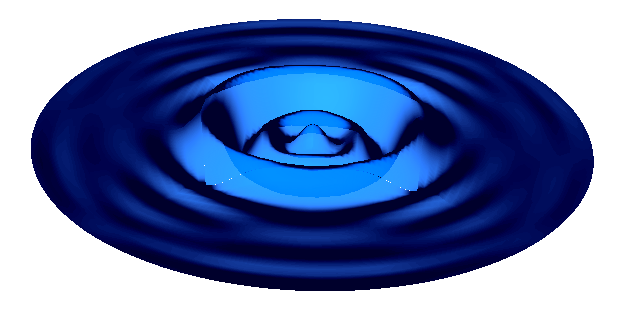
\includegraphics[width=0.25\textwidth]{images/shallowWater.png}}
}


\author{Joseph Schoonover}
\date{}

\begin{document}
\frontmatter
% Doing a custom title-page
\begin{titlingpage}
    
        \vspace*{2cm}

   % Setup up the main and sub-titles with the logo
   {\fontfamily{cmss}\selectfont
   \begin{center}
     \HUGE{\textbf{ Spectral Element Libraries in Fortran (SELF) }}\\

     \huge{\textbf{\textcolor{blue}{Barotropic, Geostrophic Circulation}}}
     \huge{\textit{\textcolor{blue}{Steady State Solver}}}
   \end{center}
    }    
 
        \vspace{1cm}
        
%        \begin{center}
%         \swlogo
%        \end{center}
        
        \vspace{2cm}
        
     \begin{center}
     
        %Do a subtitle here if you like
        {\fontfamily{cmss}\selectfont
        \huge{
           Reference Manual
        }
        
        \vspace{1.5cm}
        
        % Enter the author's name
        \textbf{
        \large{
           \theauthor 
         }}}
        
        \vfill
        
        
     \end{center}
        
    
\end{titlingpage}


{\fontfamily{cmss}\selectfont
\tableofcontents
}
\mainmatter

% Special Style
\pagestyle{myheadings}

\chapter{Equations and Discretization}
The dynamics of the large scale oceanic circulation on earth are largely contained within the hydrostatic primitive equations. In these equations, the vertical momentum balance is approximated by hyrdostatic balance - an approximation that is justified by the use of the ``thin shell'' approximation, where the fluid depth is far smaller than the lateral length scales of motion. For a constant density fluid, the hydrostatic primitive equations can be reduced to the shallow water equations, so long as the effects of thin boundary layers are parameterized. For sufficiently slow moving flows, the effects of gravity waves can be approximated as instantaneous adjustments of the fluid surface that act to keep the fluid transport divergence free; this is known as the rigid lid assumption. Steady state, linear flows subject to all of the previous assumptions are now governed by two equations :
\begin{subequations}
\begin{align}
  f \hat{z} \times \vec{u} &= \nabla P + \frac{ \vec{\tau} }{H} - \frac{C_d \vec{u}}{H} \\
  \nabla \cdot \left( H \vec{u} \right) &= 0.
\end{align}\label{eq:eqofmotion}
\end{subequations}
In Eqs. \eqref{eq:eqofmotion}, $f$ is the coriolis parameter, $\vec{u} = u \hat{x} + v\hat{y}$ is the lateral velocity field, $P$ is the barotropic fluid pressure, $\vec{\tau}$ is the stress imposed on the fluid at the surface, $C_d\vec{u}$ is a parameterization of the stress felt at the sea-floor, $C_d$ is a drag coefficient, and $H$ is the fluid depth.

Eq. (\ref{eq:eqofmotion}b) is satisfied exactly if the transport is written in terms of a stream function
\begin{equation}
H \vec{u} = \hat{z} \times \nabla \Psi. \label{eq:stream}
\end{equation}
Further, the equation set \eqref{eq:eqofmotion} can be reduced to a single equation for the stream function by taking the curl of (\ref{eq:eqofmotion}a) and substituting in \eqref{eq:stream}. Doing so gives
\begin{equation}
 \nabla \cdot \left( \frac{C_d \nabla \Psi}{H^2} \right) + \nabla \Psi \times \nabla Q = \nabla \times \left( \frac{\vec{\tau}}{H} \right) ,\label{eq:eqsolved}
\end{equation} 
where 
\begin{equation}
Q = \frac{f}{H}
\end{equation}
is the background potential vorticity.


\section{Nodal Continuous Galerkin Discretization}


\section{Iterative Solution Technique}
The discretized drag operator is symmetric, while the potential vorticity advection operator is asymmetric. Overall, the system is asymmetric. Previous implementation of the SELF-CGSEM solver make use of the preconditioned conjugate gradient method, an iterative solver that is not directly applicable to asymmetric systems

\clearpage

\appendix

\chapter{Spectral Element Primer}

\section{Vector Spaces}


\section{Spectral Approximations and Error Analysis}

\chapter{Differential Geometry}\label{chap:GeometryTheory}

\pagebreak

\bibliography{hpe-refs}
\bibliographystyle{plainnat}
\end{document}